%% This file was auto-generated by IPython.
%% Conversion from the original notebook file:
%% stat_hadoop_logreg2.ipynb
%%
\documentclass[11pt,english,fleqn]{article}

%% This is the automatic preamble used by IPython.  Note that it does *not*
%% include a documentclass declaration, that is added at runtime to the overall
%% document.

\usepackage{amsmath}
\usepackage{amssymb}
\usepackage{graphicx}
\usepackage{ucs}
\usepackage[utf8x]{inputenc}

% needed for markdown enumerations to work
\usepackage{enumerate}

% Slightly bigger margins than the latex defaults
\usepackage{geometry}
\geometry{verbose,tmargin=3cm,bmargin=3cm,lmargin=2.5cm,rmargin=2.5cm}

% Define a few colors for use in code, links and cell shading
\usepackage{color}
\definecolor{orange}{cmyk}{0,0.4,0.8,0.2}
\definecolor{darkorange}{rgb}{.71,0.21,0.01}
\definecolor{darkgreen}{rgb}{.12,.54,.11}
\definecolor{myteal}{rgb}{.26, .44, .56}
\definecolor{gray}{gray}{0.45}
\definecolor{lightgray}{gray}{.95}
\definecolor{mediumgray}{gray}{.8}
\definecolor{inputbackground}{rgb}{.95, .95, .85}
\definecolor{outputbackground}{rgb}{.95, .95, .95}
\definecolor{traceback}{rgb}{1, .95, .95}

% Framed environments for code cells (inputs, outputs, errors, ...).  The
% various uses of \unskip (or not) at the end were fine-tuned by hand, so don't
% randomly change them unless you're sure of the effect it will have.
\usepackage{framed}

% remove extraneous vertical space in boxes
\setlength\fboxsep{0pt}

% codecell is the whole input+output set of blocks that a Code cell can
% generate.

% TODO: unfortunately, it seems that using a framed codecell environment breaks
% the ability of the frames inside of it to be broken across pages.  This
% causes at least the problem of having lots of empty space at the bottom of
% pages as new frames are moved to the next page, and if a single frame is too
% long to fit on a page, will completely stop latex from compiling the
% document.  So unless we figure out a solution to this, we'll have to instead
% leave the codecell env. as empty.  I'm keeping the original codecell
% definition here (a thin vertical bar) for reference, in case we find a
% solution to the page break issue.

%% \newenvironment{codecell}{%
%%     \def\FrameCommand{\color{mediumgray} \vrule width 1pt \hspace{5pt}}%
%%    \MakeFramed{\vspace{-0.5em}}}
%%  {\unskip\endMakeFramed}

% For now, make this a no-op...
\newenvironment{codecell}{}

 \newenvironment{codeinput}{%
   \def\FrameCommand{\colorbox{inputbackground}}%
   \MakeFramed{\advance\hsize-\width \FrameRestore}}
 {\unskip\endMakeFramed}

\newenvironment{codeoutput}{%
   \def\FrameCommand{\colorbox{outputbackground}}%
   \vspace{-1.4em}
   \MakeFramed{\advance\hsize-\width \FrameRestore}}
 {\unskip\medskip\endMakeFramed}

\newenvironment{traceback}{%
   \def\FrameCommand{\colorbox{traceback}}%
   \MakeFramed{\advance\hsize-\width \FrameRestore}}
 {\endMakeFramed}

% Use and configure listings package for nicely formatted code
\usepackage{listingsutf8}
\lstset{
  language=python,
  inputencoding=utf8x,
  extendedchars=\true,
  aboveskip=\smallskipamount,
  belowskip=\smallskipamount,
  xleftmargin=2mm,
  breaklines=true,
  basicstyle=\small \ttfamily,
  showstringspaces=false,
  keywordstyle=\color{blue}\bfseries,
  commentstyle=\color{myteal},
  stringstyle=\color{darkgreen},
  identifierstyle=\color{darkorange},
  columns=fullflexible,  % tighter character kerning, like verb
}

% The hyperref package gives us a pdf with properly built
% internal navigation ('pdf bookmarks' for the table of contents,
% internal cross-reference links, web links for URLs, etc.)
\usepackage{hyperref}
\hypersetup{
  breaklinks=true,  % so long urls are correctly broken across lines
  colorlinks=true,
  urlcolor=blue,
  linkcolor=darkorange,
  citecolor=darkgreen,
  }

% hardcode size of all verbatim environments to be a bit smaller
\makeatletter 
\g@addto@macro\@verbatim\small\topsep=0.5em\partopsep=0pt
\makeatother 

% Prevent overflowing lines due to urls and other hard-to-break entities.
\sloppy

\setlength{\mathindent}{0pt}
\setlength{\parindent}{0pt}
\setlength{\parskip}{8pt}
\begin{document}

\section{Paralel Lojistik Regresyon, Esle/Indirge}

Lojistik regresyon kodunu esle-indirge (map-reduce) uzerinden paralelize
etmek icin literature {[}1-7{]} bakinca, genel yaklasimin makinalara
bolunen veri parcalari uzerinde ayri ayri graydan cikisinin (gradient
ascent) isletilmesi ve sonuc $\theta$'larin son bir makinada
ortalamasinin alinmasi oldugunu goruruz.

Daha onceki \emph{lojistik regresyon} yazimizda iki farkli gradyan cikis
algoritmasi gormustuk. Bu algoritmalardan kullanacagimiz daha basit
olani, her dongude alpha'yi degistiren versiyon degil tek alpha
kullanan, ve kod icinde zar atan degil, veriyi sirayla isleyen. Bunun
birkac sebebi var, oncelikle altta gorecegimiz uzere veriyi Hadoop'a
vermeden once kendimiz karistiracagiz, yani kod icinde zar atmaya gerek
kalmayacak. Ikincisi pek cok makinada islem yapildigi icin tek bir sabit
uzerinden azaltma yapmak mumkun degil (fakat her isleyicinin
-degismeyen- kendine has / ayri bir sabiti olabilir, bu konuyu ileride
isleyebiliriz), bu sebeple ve basitlik amaciyla tek sabitli kod
kullanildi. Ayrica artik dongu (iterasyon) yok, yani veri bastan sona
bir kez tarandi mi, o makinanin islemi bitecek. Fakat buyuk veri
ortaminda (ki zaten onun icin Hadoop kullaniyoruz herhalde) elimizde o
kadar cok veri olacak ki bu verinin tamamini isleyince zaten 100,200
kere donguyu isletmek ile ayni etkiyi almis oluyoruz.

Ornek veri olarak alttakini urettik,

\begin{codecell}
\begin{codeinput}
\begin{lstlisting}
from pandas import *
mean1 = [10,10]
mean2 = [20,20]
cov = [[5,0],[0,5]]
d1 = DataFrame(np.random.multivariate_normal(mean1,cov,10000))
d2 = DataFrame(np.random.multivariate_normal(mean2,cov,10000))
d1['labels'] = 1
d2['labels'] = 0
data = DataFrame(np.vstack((d1,d2)))
data.to_csv("testSet.txt",sep='\t',index=None,header=None)
print data[:4]

\end{lstlisting}
\end{codeinput}
\begin{codeoutput}
\begin{verbatim}
0          1  2
0  7.327967   7.730789  1
1  7.693445   7.305714  1
2  6.818491  10.632738  1
3  7.305205   8.551828  1
\end{verbatim}
\end{codeoutput}
\end{codecell}
\begin{codecell}
\begin{codeinput}
\begin{lstlisting}
plt.plot(d1.ix[:,0],d1.ix[:,1],'b.')
plt.hold(True)
plt.plot(d2.ix[:,0],d2.ix[:,1],'r.')
plt.hold(True)

\end{lstlisting}
\end{codeinput}
\begin{codeoutput}
\begin{center}
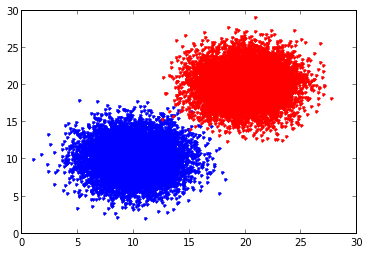
\includegraphics[width=0.7\textwidth]{stat_hadoop_logreg2_files/stat_hadoop_logreg2_fig_00.png}
\par
\end{center}
\end{codeoutput}
\end{codecell}
Hadoop'u baslatalim,

\begin{codecell}
\begin{codeinput}
\begin{lstlisting}
!ssh localhost -l hduser $HOME/Downloads/hadoop*/bin/stop-all.sh
!ssh localhost -l hduser $HOME/Downloads/hadoop*/bin/start-all.sh

\end{lstlisting}
\end{codeinput}
\begin{codeoutput}
\begin{verbatim}
no jobtracker to stop
\end{verbatim}
\begin{verbatim}
localhost: no tasktracker to stop
\end{verbatim}
\begin{verbatim}
no namenode to stop
\end{verbatim}
\begin{verbatim}
localhost: no datanode to stop
\end{verbatim}
\begin{verbatim}
localhost: no secondarynamenode to stop
\end{verbatim}
\begin{verbatim}
starting namenode, logging to /home/burak/Downloads/hadoop-1.2.1/libexec/../logs/hadoop-hduser-namenode-burak-Aspire-S3.out
\end{verbatim}
\begin{verbatim}
localhost: starting datanode, logging to /home/burak/Downloads/hadoop-1.2.1/libexec/../logs/hadoop-hduser-datanode-burak-Aspire-S3.out
\end{verbatim}
\begin{verbatim}
localhost: starting secondarynamenode, logging to /home/burak/Downloads/hadoop-1.2.1/libexec/../logs/hadoop-hduser-secondarynamenode-burak-Aspire-S3.out
\end{verbatim}
\begin{verbatim}
starting jobtracker, logging to /home/burak/Downloads/hadoop-1.2.1/libexec/../logs/hadoop-hduser-jobtracker-burak-Aspire-S3.out
\end{verbatim}
\begin{verbatim}
localhost: starting tasktracker, logging to /home/burak/Downloads/hadoop-1.2.1/libexec/../logs/hadoop-hduser-tasktracker-burak-Aspire-S3.out
\end{verbatim}
\end{codeoutput}
\end{codecell}
Altta veriyi isletmeden once kendimiz karistiriyoruz,

\begin{codecell}
\begin{codeinput}
\begin{lstlisting}
!sort --random-sort testSet.txt > /tmp/testSet1.txt

\end{lstlisting}
\end{codeinput}
\end{codecell}
\begin{codecell}
\begin{codeinput}
\begin{lstlisting}
print open("logreg.py").read()
\end{lstlisting}
\end{codeinput}
\begin{codeoutput}
\begin{verbatim}
'''
Logistic regression for map/reduce written for MRJob,
uses stochastic gradient descent.
'''
from mrjob.job import MRJob
from mrjob.protocol import PickleProtocol
import numpy as np
import os, thread

class MRLogisticRegression(MRJob):
    INTERNAL_PROTOCOL = PickleProtocol
    
    def __init__(self, *args, **kwargs):
        super(MRLogisticRegression, self).__init__(*args, **kwargs)
        self.n  = 1
        self.m = 3
        self.count = 0
        self.theta = np.ones((self.m,1))
        self.final_theta = np.zeros((self.m,self.n))

    def sigmoid(self, arr):
        return 1.0/(1+np.exp(-arr))

    def stoc_grad_ascent0(self, data_mat, label, theta):
        alpha = 0.01
        for j in range(self.m):
            h = self.sigmoid(np.dot(data_mat,theta)[0])
            theta[j] = theta[j] + alpha * data_mat[j] * (label - h)
        return theta
        
    def mapper(self, key, line):        
        tokens = map(np.float,line.split('\t'))
        data = np.append(1.0,np.array(tokens[:-1]))
        label = np.array(tokens[-1])
        self.theta = self.stoc_grad_ascent0(data, label, self.theta)
        
    def mapper_final(self):        
        yield ("key1", self.theta)
                
    def reducer(self, key, tokens):
        for val in tokens:
            self.final_theta += val
            self.count += 1
        yield('result',str(self.final_theta / self.count))
        
if __name__ == '__main__':
    MRLogisticRegression.run()
\end{verbatim}
\end{codeoutput}
\end{codecell}
Ustte esleyici icinde tek bir tane anahtar uretiyoruz, tum makinalarda
tum esleyiciler ayni anahtari, bir kez uretiyor olacaklar. Bunun sebebi
nedir? Ne yapmaya calistigimizi hatirlayalim, tum makinalarda lojistik
regresyon isletiyoruz, gradyan cikisi yapiyoruz, ve sonucta o makinanin
isi bitince elimizde tek bir tane agirlik vektoru yani theta olacak.
Ilgilendigimiz sonuc bu, o yuzden cikti stdout'a tek bir satir
yaziliyor. Peki niye ayni anahtar? Cunku her makinadaki tum agirlik
vektorlerinin ``hep beraber'' bir noktada ortalamasinin alinmasini
istiyoruz, bunu Hadoop'a yaptirmanin bir yolu herkese ayni anahtari
kullandirtmak, boylece bu anahtarlar tek bir indirgeyiciye (ve makinaya)
gidecek, ve orada ortalamalari alinacak. Tum esleyicilerin sonucunun tek
bir indirgeciye gitmesi performans problemi cikartmaz mi? Cikmaz, cunku
1000 tane, 10000 tane esleyici paralel is yapmis olabilir, ama isleri
bitince elimizde 1000,10000 tane agirlik vektoru olacak, ve bu zaten tek
makinanin rahatlikla basa cikabilecegi bir yuktur.

Bu yaklasim, esleyicinin her veri satiri basina bir ya da daha fazla
anahtar-deger satiri urettigi yaklasimdan (mesela klasik kelime sayma
problemi) biraz farkli, o sebeple bu farkliligi belirtmek istedik.

Bir puf nokta, her veri satiri icin isletilen map'e de aslinda anahtar
urettirmiyoruz, tum map cagrilari bittikten sonra son bir kez
cagirilacak map\_final'a bu isi yaptiriyoruz. Oraya gelinceye kadar (map
icinde) degisen theta'yi surekli hafizada tutmusuz, son noktaya gelince
o sonucu ayni anahtar ile esleyerek uretiyoruz ve is bitiyor.

Komut satirindan isletelim:

\begin{codecell}
\begin{codeinput}
\begin{lstlisting}
!python $HOME/Documents/classnotes/stat/stat_hadoop_logreg/logreg.py /tmp/testSet1.txt

\end{lstlisting}
\end{codeinput}
\begin{codeoutput}
\begin{verbatim}
using configs in /home/burak/.mrjob.conf
creating tmp directory /tmp/logreg.burak.20130817.060556.092720
writing to step-0-mapper_part-00000
\end{verbatim}
\begin{verbatim}
Counters from step 1:
  (no counters found)
writing to /tmp/logreg.burak.20130817.060556.092720/step-0-mapper-sorted
> sort /tmp/logreg.burak.20130817.060556.092720/step-0-mapper_part-00000
writing to step-0-reducer_part-00000
Counters from step 1:
  (no counters found)
Moving /tmp/logreg.burak.20130817.060556.092720/step-0-reducer_part-00000 -> /tmp/logreg.burak.20130817.060556.092720/output/part-00000
Streaming final output from /tmp/logreg.burak.20130817.060556.092720/output
"result"	"[[ 9.50829527]\n [-0.36317422]\n [-0.34354905]]"
removing tmp directory /tmp/logreg.burak.20130817.060556.092720
\end{verbatim}
\end{codeoutput}
\end{codecell}
\begin{codecell}
\begin{codeinput}
\begin{lstlisting}
def plot_theta(theta):
    x = np.array(arange(-10.0, 40.0, 0.1))
    y = np.array((-theta[0]-theta[1]*x)/theta[2])
    plot(x, y)
    hold(True)
    plot(d1.ix[:,0],d1.ix[:,1],'b.')
    hold(True)
    plot(d2.ix[:,0],d2.ix[:,1],'r.')
    hold(True)
    ylim(0,30)
    xlim(0,30)

theta = [9.50829527,-0.36317422,-0.34354905]
plot_theta(theta)
\end{lstlisting}
\end{codeinput}
\begin{codeoutput}
\begin{center}
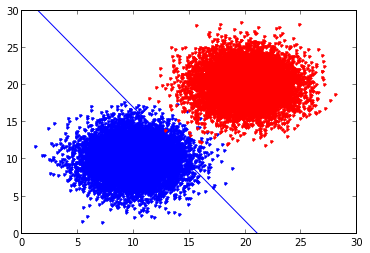
\includegraphics[width=0.7\textwidth]{stat_hadoop_logreg2_files/stat_hadoop_logreg2_fig_01.png}
\par
\end{center}
\end{codeoutput}
\end{codecell}
\subsection{Hadoop Kullanarak}


Dosyalari kopyalayalim

\begin{codecell}
\begin{codeinput}
\begin{lstlisting}
!ssh localhost -l hduser $HOME/Downloads/hadoop*/bin/hadoop dfs -rmr /user/testSet1.txt
!ssh localhost -l hduser $HOME/Downloads/hadoop*/bin/hadoop dfs -copyFromLocal /tmp/testSet1.txt /user

\end{lstlisting}
\end{codeinput}
\begin{codeoutput}
\begin{verbatim}
Deleted hdfs://localhost:54310/user/testSet1.txt
\end{verbatim}
\end{codeoutput}
\end{codecell}
Iki tane esleyici iki tane indirgeyici olmak uzere Hadoop uzerinden ayni
islemi yapalim.

\begin{codecell}
\begin{codeinput}
\begin{lstlisting}
!ssh localhost -l hduser python $HOME/Documents/classnotes/stat/stat_hadoop_logreg/logreg.py hdfs:///user/testSet1.txt -r hadoop --step-num=1 --jobconf mapred.map.tasks=2 --jobconf mapred.reduce.tasks=2
 
\end{lstlisting}
\end{codeinput}
\begin{codeoutput}
\begin{verbatim}
using configs in /home/hduser/.mrjob.conf
creating tmp directory /tmp/logreg.hduser.20130817.060935.871133
\end{verbatim}
\begin{verbatim}
Copying local files into hdfs:///user/hduser/tmp/mrjob/logreg.hduser.20130817.060935.871133/files/
\end{verbatim}
\begin{verbatim}
Using Hadoop version 1.2.1
\end{verbatim}
\begin{verbatim}
HADOOP: packageJobJar: [/app/hadoop/tmp/hadoop-unjar5290319381457678871/] [] /tmp/streamjob5226598311088374006.jar tmpDir=null

HADOOP: Loaded the native-hadoop library

HADOOP: Snappy native library not loaded

HADOOP: Total input paths to process : 1

HADOOP: getLocalDirs(): [/app/hadoop/tmp/mapred/local]

HADOOP: Running job: job_201308170806_0002

HADOOP: To kill this job, run:

HADOOP: /home/burak/Downloads/hadoop-1.2.1/libexec/../bin/hadoop job  -Dmapred.job.tracker=localhost:54311 -kill job_201308170806_0002

HADOOP: Tracking URL: http://localhost:50030/jobdetails.jsp?jobid=job_201308170806_0002

HADOOP:  map 0%  reduce 0%

HADOOP:  map 100%  reduce 0%

HADOOP:  map 100%  reduce 17%

HADOOP:  map 100%  reduce 33%

HADOOP:  map 100%  reduce 67%

HADOOP:  map 100%  reduce 100%

HADOOP: Job complete: job_201308170806_0002

HADOOP: Output: hdfs:///user/hduser/tmp/mrjob/logreg.hduser.20130817.060935.871133/output

Counters from step 1:
  File Input Format Counters :
    Bytes Read: 823345
  File Output Format Counters :
    Bytes Written: 59
  FileSystemCounters:
    FILE_BYTES_READ: 638
    FILE_BYTES_WRITTEN: 242936
    HDFS_BYTES_READ: 823531
    HDFS_BYTES_WRITTEN: 59
  Job Counters :
    Data-local map tasks: 2
    Launched map tasks: 2
    Launched reduce tasks: 2
    SLOTS_MILLIS_MAPS: 10130
    SLOTS_MILLIS_REDUCES: 19695
    Total time spent by all maps waiting after reserving slots (ms): 0
    Total time spent by all reduces waiting after reserving slots (ms): 0
  Map-Reduce Framework:
    CPU time spent (ms): 3870
    Combine input records: 0
    Combine output records: 0
    Map input bytes: 819298
    Map input records: 20000
    Map output bytes: 618
    Map output materialized bytes: 650
    Map output records: 2
    Physical memory (bytes) snapshot: 579891200
    Reduce input groups: 1
    Reduce input records: 2
    Reduce output records: 1
    Reduce shuffle bytes: 650
    SPLIT_RAW_BYTES: 186
    Spilled Records: 4
    Total committed heap usage (bytes): 435814400
    Virtual memory (bytes) snapshot: 4310802432
Streaming final output from hdfs:///user/hduser/tmp/mrjob/logreg.hduser.20130817.060935.871133/output
\end{verbatim}
\begin{verbatim}
"result"	"[[ 7.38405717]\n [-0.26595013]\n [-0.26421385]]"
removing tmp directory /tmp/logreg.hduser.20130817.060935.871133
deleting hdfs:///user/hduser/tmp/mrjob/logreg.hduser.20130817.060935.871133 from HDFS
\end{verbatim}
\end{codeoutput}
\end{codecell}
\begin{codecell}
\begin{codeinput}
\begin{lstlisting}
theta = [7.38405717,-0.26595013,-0.26421385]
plot_theta(theta)
\end{lstlisting}
\end{codeinput}
\begin{codeoutput}
\begin{center}
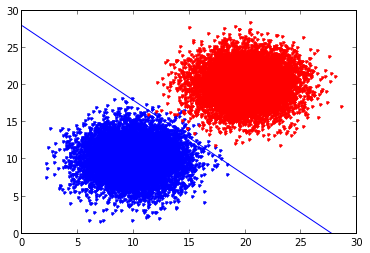
\includegraphics[width=0.7\textwidth]{stat_hadoop_logreg2_files/stat_hadoop_logreg2_fig_02.png}
\par
\end{center}
\end{codeoutput}
\end{codecell}
Kaynaklar

{[}1{]} http://alex.smola.org/teaching/berkeley2012/slides/4
Optimization.pdf

{[}2{]} http://cs.kangwon.ac.kr/∼ysmoon/courses/2011 1/grad
mining/slides/07-2.pdf

{[}3{]} http://www.slideshare.net/hadoop/modeling-with-hadoop-kdd2011

{[}4{]}
http://www.xmarks.com/site/www.cs.stanford.edu/people/ang/papers/nips06-mapreducemulticore.pdf

{[}5{]} http://books.nips.cc/papersnips23/NIPS2010 1162.pdf

{[}6{]} http://simianer.de/P12-1002-slides.pdf

{[}7{]} http://www.holehouse.org/mlclass/17 Large Scale Machine
Learning.html

{[}8{]}
https://github.com/elsevierlabs/logistic-regression-sgd-mapreduce

\end{document}
